\chapter{Data Understanding}

\section{Data Sources}
The project leverages two distinct datasets to address the diagnosis and prognosis objectives respectively.

\subsection{WBCD Dataset (Diagnosis)}
The \textbf{Wisconsin Breast Cancer Diagnosis (WBCD)} dataset is a standard benchmark in medical machine learning. It consists of features computed from a digitized image of a fine needle aspirate (FNA) of a breast mass.
\begin{itemize}
    \item \textbf{Instances:} 569
    \item \textbf{Features:} 30 real-valued features (radius, texture, perimeter, area, smoothness, compactness, concavity, concave points, symmetry, and fractal dimension).
    \item \textbf{Target:} Diagnosis (M = Malignant, B = Benign).
\end{itemize}

\subsection{METABRIC Dataset (Prognosis)}
The \textbf{Molecular Taxonomy of Breast Cancer International Consortium (METABRIC)} dataset provides clinical and genomic data for breast cancer patients.
\begin{itemize}
    \item \textbf{Usage:} Used here for the regression task to predict tumor characteristics and patient outcomes.
    \item \textbf{Key Features:} Clinical attributes such as age, tumor size, lymph nodes, and gene expression data.
\end{itemize}

\section{Exploratory Data Analysis (EDA)}

\subsection{WBCD Exploratory Analysis}
This section details the exploratory analysis performed on the Wisconsin Breast Cancer Diagnosis (WBCD) dataset.

\subsubsection{Dimensions and Data Types}
The dataset consists of 569 instances and 32 columns.
\begin{itemize}
    \item \textbf{ID}: Unique identifier (Integer).
    \item \textbf{Diagnosis}: Target variable (Object: 'M' for Malignant, 'B' for Benign).
    \item \textbf{Features}: 30 real-valued input features (Float64) describing cell nucleus characteristics.
    \item \textbf{Unnamed: 32}: Artifact column containing null values.
\end{itemize}

\subsubsection{Descriptive Statistics}
Key statistical measures for representative features are summarized below. The scale differences (e.g., Area $\approx$ 650 vs Smoothness $\approx$ 0.1) indicate the need for feature scaling (Standardization) during preprocessing.

\begin{table}[H]
\centering
\renewcommand{\arraystretch}{0.9} % Reduce row height
\scalebox{0.92}{ % Scale down the entire table
\begin{tabular}{|l|c|c|c|c|}
\hline
\textbf{Feature} & \textbf{Mean} & \textbf{Std Dev} & \textbf{Min} & \textbf{Max} \\ \hline
radius\_mean & 14.127 & 3.524 & 6.981 & 28.110 \\ \hline
texture\_mean & 19.290 & 4.301 & 9.710 & 39.280 \\ \hline
perimeter\_mean & 91.969 & 24.299 & 43.790 & 188.500 \\ \hline
area\_mean & 654.889 & 351.914 & 143.500 & 2501.000 \\ \hline
smoothness\_mean & 0.096 & 0.014 & 0.053 & 0.163 \\ \hline
compactness\_mean & 0.104 & 0.053 & 0.019 & 0.345 \\ \hline
concavity\_mean & 0.089 & 0.080 & 0.000 & 0.427 \\ \hline
concave\_points\_mean & 0.049 & 0.039 & 0.000 & 0.201 \\ \hline
symmetry\_mean & 0.181 & 0.027 & 0.106 & 0.304 \\ \hline
fractal\_dimension\_mean & 0.063 & 0.007 & 0.050 & 0.097 \\ \hline
radius\_se & 0.405 & 0.277 & 0.112 & 2.873 \\ \hline
texture\_se & 1.217 & 0.552 & 0.360 & 4.885 \\ \hline
perimeter\_se & 2.866 & 2.022 & 0.757 & 21.980 \\ \hline
area\_se & 40.337 & 45.491 & 6.802 & 542.200 \\ \hline
smoothness\_se & 0.007 & 0.003 & 0.002 & 0.031 \\ \hline
compactness\_se & 0.025 & 0.018 & 0.002 & 0.135 \\ \hline
concavity\_se & 0.032 & 0.030 & 0.000 & 0.396 \\ \hline
concave\_points\_se & 0.012 & 0.006 & 0.000 & 0.053 \\ \hline
symmetry\_se & 0.021 & 0.008 & 0.008 & 0.079 \\ \hline
fractal\_dimension\_se & 0.004 & 0.003 & 0.001 & 0.030 \\ \hline
radius\_worst & 16.269 & 4.833 & 7.930 & 36.040 \\ \hline
texture\_worst & 25.677 & 6.146 & 12.020 & 49.540 \\ \hline
perimeter\_worst & 107.261 & 33.603 & 50.410 & 251.200 \\ \hline
area\_worst & 880.583 & 569.357 & 185.200 & 4254.000 \\ \hline
smoothness\_worst & 0.132 & 0.023 & 0.071 & 0.223 \\ \hline
compactness\_worst & 0.254 & 0.157 & 0.027 & 1.058 \\ \hline
concavity\_worst & 0.272 & 0.209 & 0.000 & 1.252 \\ \hline
concave\_points\_worst & 0.115 & 0.066 & 0.000 & 0.291 \\ \hline
symmetry\_worst & 0.290 & 0.062 & 0.157 & 0.664 \\ \hline
fractal\_dimension\_worst & 0.084 & 0.018 & 0.055 & 0.207 \\ \hline
\end{tabular}
}
\caption{Descriptive Statistics for All WBCD Features}
\label{tab:wbcd_stats_full}
\end{table}

\subsubsection{Missing Value Analysis}
Analysis of the dataset confirms high data quality:
\begin{itemize}
    \item The core feature columns contain \textbf{0 missing values}.
    \item The column \texttt{Unnamed: 32} contained 100\% missing values (NaN) and was removed during preprocessing.
\end{itemize}

\subsubsection{Target Variable Distribution}
The diagnosis target variable is binary. As visualized below, the dataset exhibits a class imbalance.

\begin{figure}[H]
    \centering
    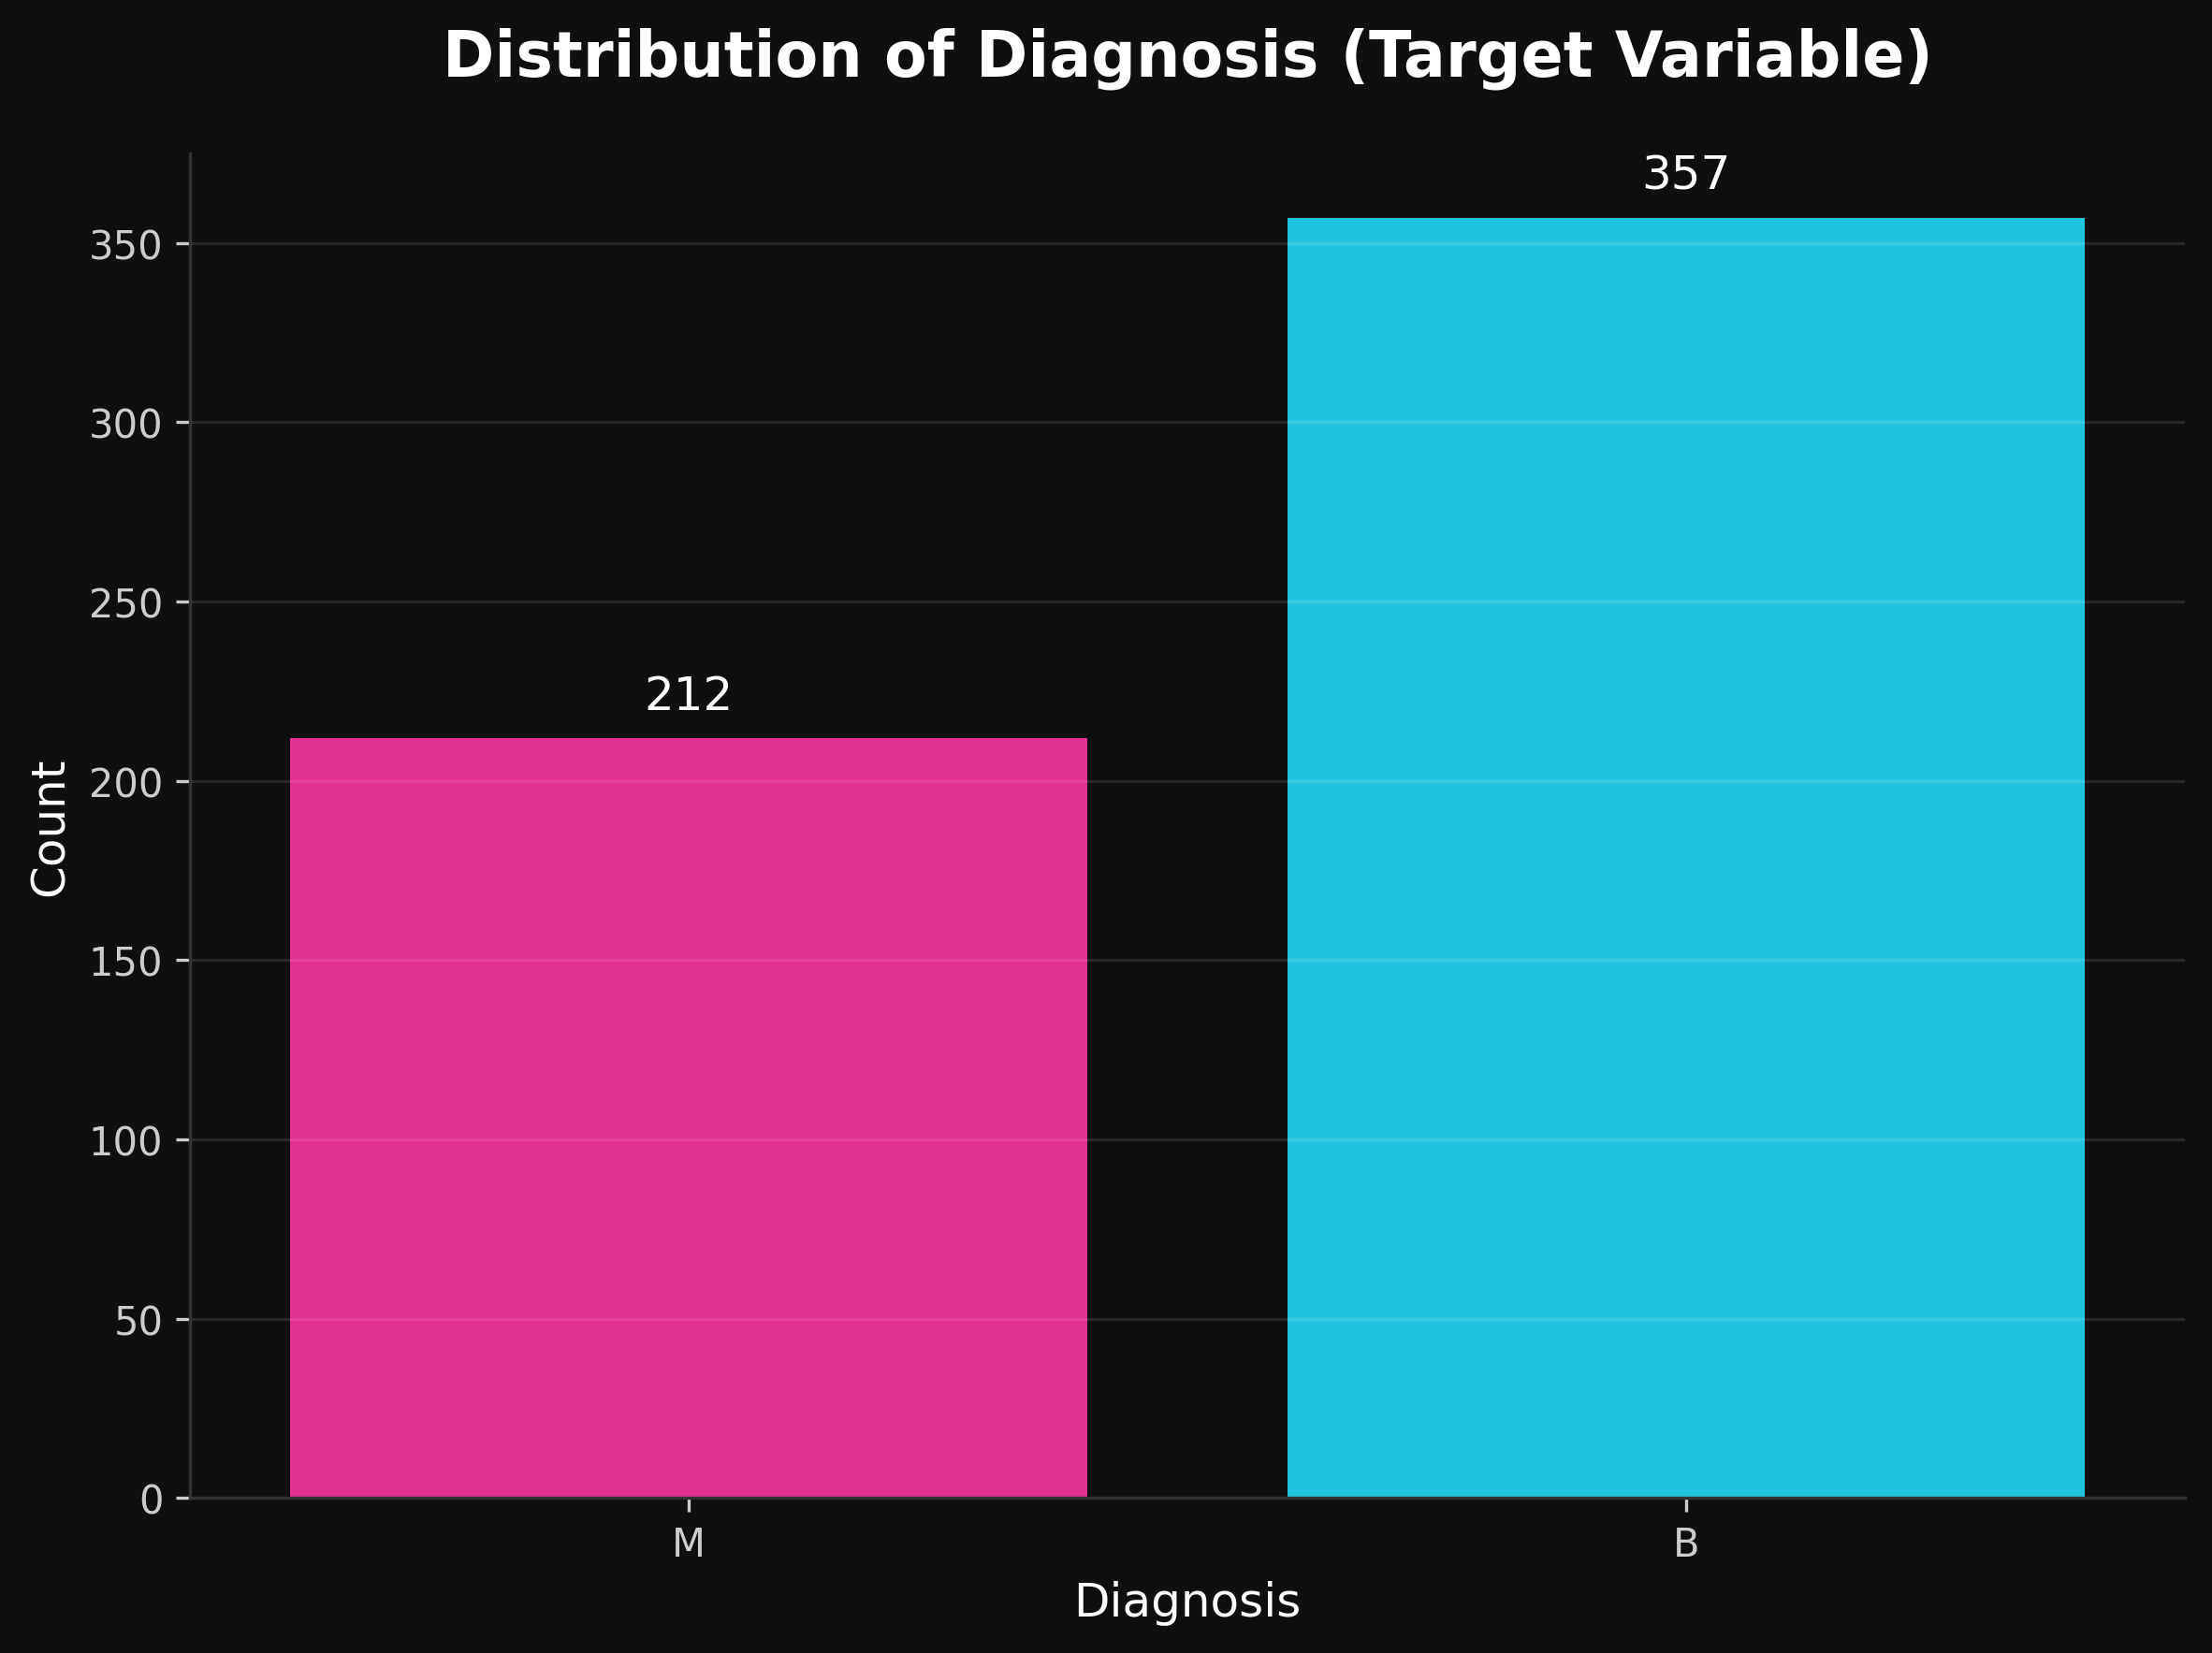
\includegraphics[width=0.7\textwidth]{images/wbcd_target_dist.png}
    \caption{Distribution of Diagnosis in WBCD Dataset}
    \label{fig:wbcd_target_dist}
\end{figure}

The majority of cases are Benign (Cyan), while Malignant cases (Pink) constitute approximately 37\% of the data. This imbalance necessitates the use of stratified sampling and specific evaluation metrics like F1-score and Sensitivity, rather than simple Accuracy.

\subsubsection{Feature Linearity and Correlation Analysis}
To identify the most predictive features, we analyzed the correlation of each feature with the target variable (encoded as Malignant=1).

\begin{figure}[H]
    \centering
    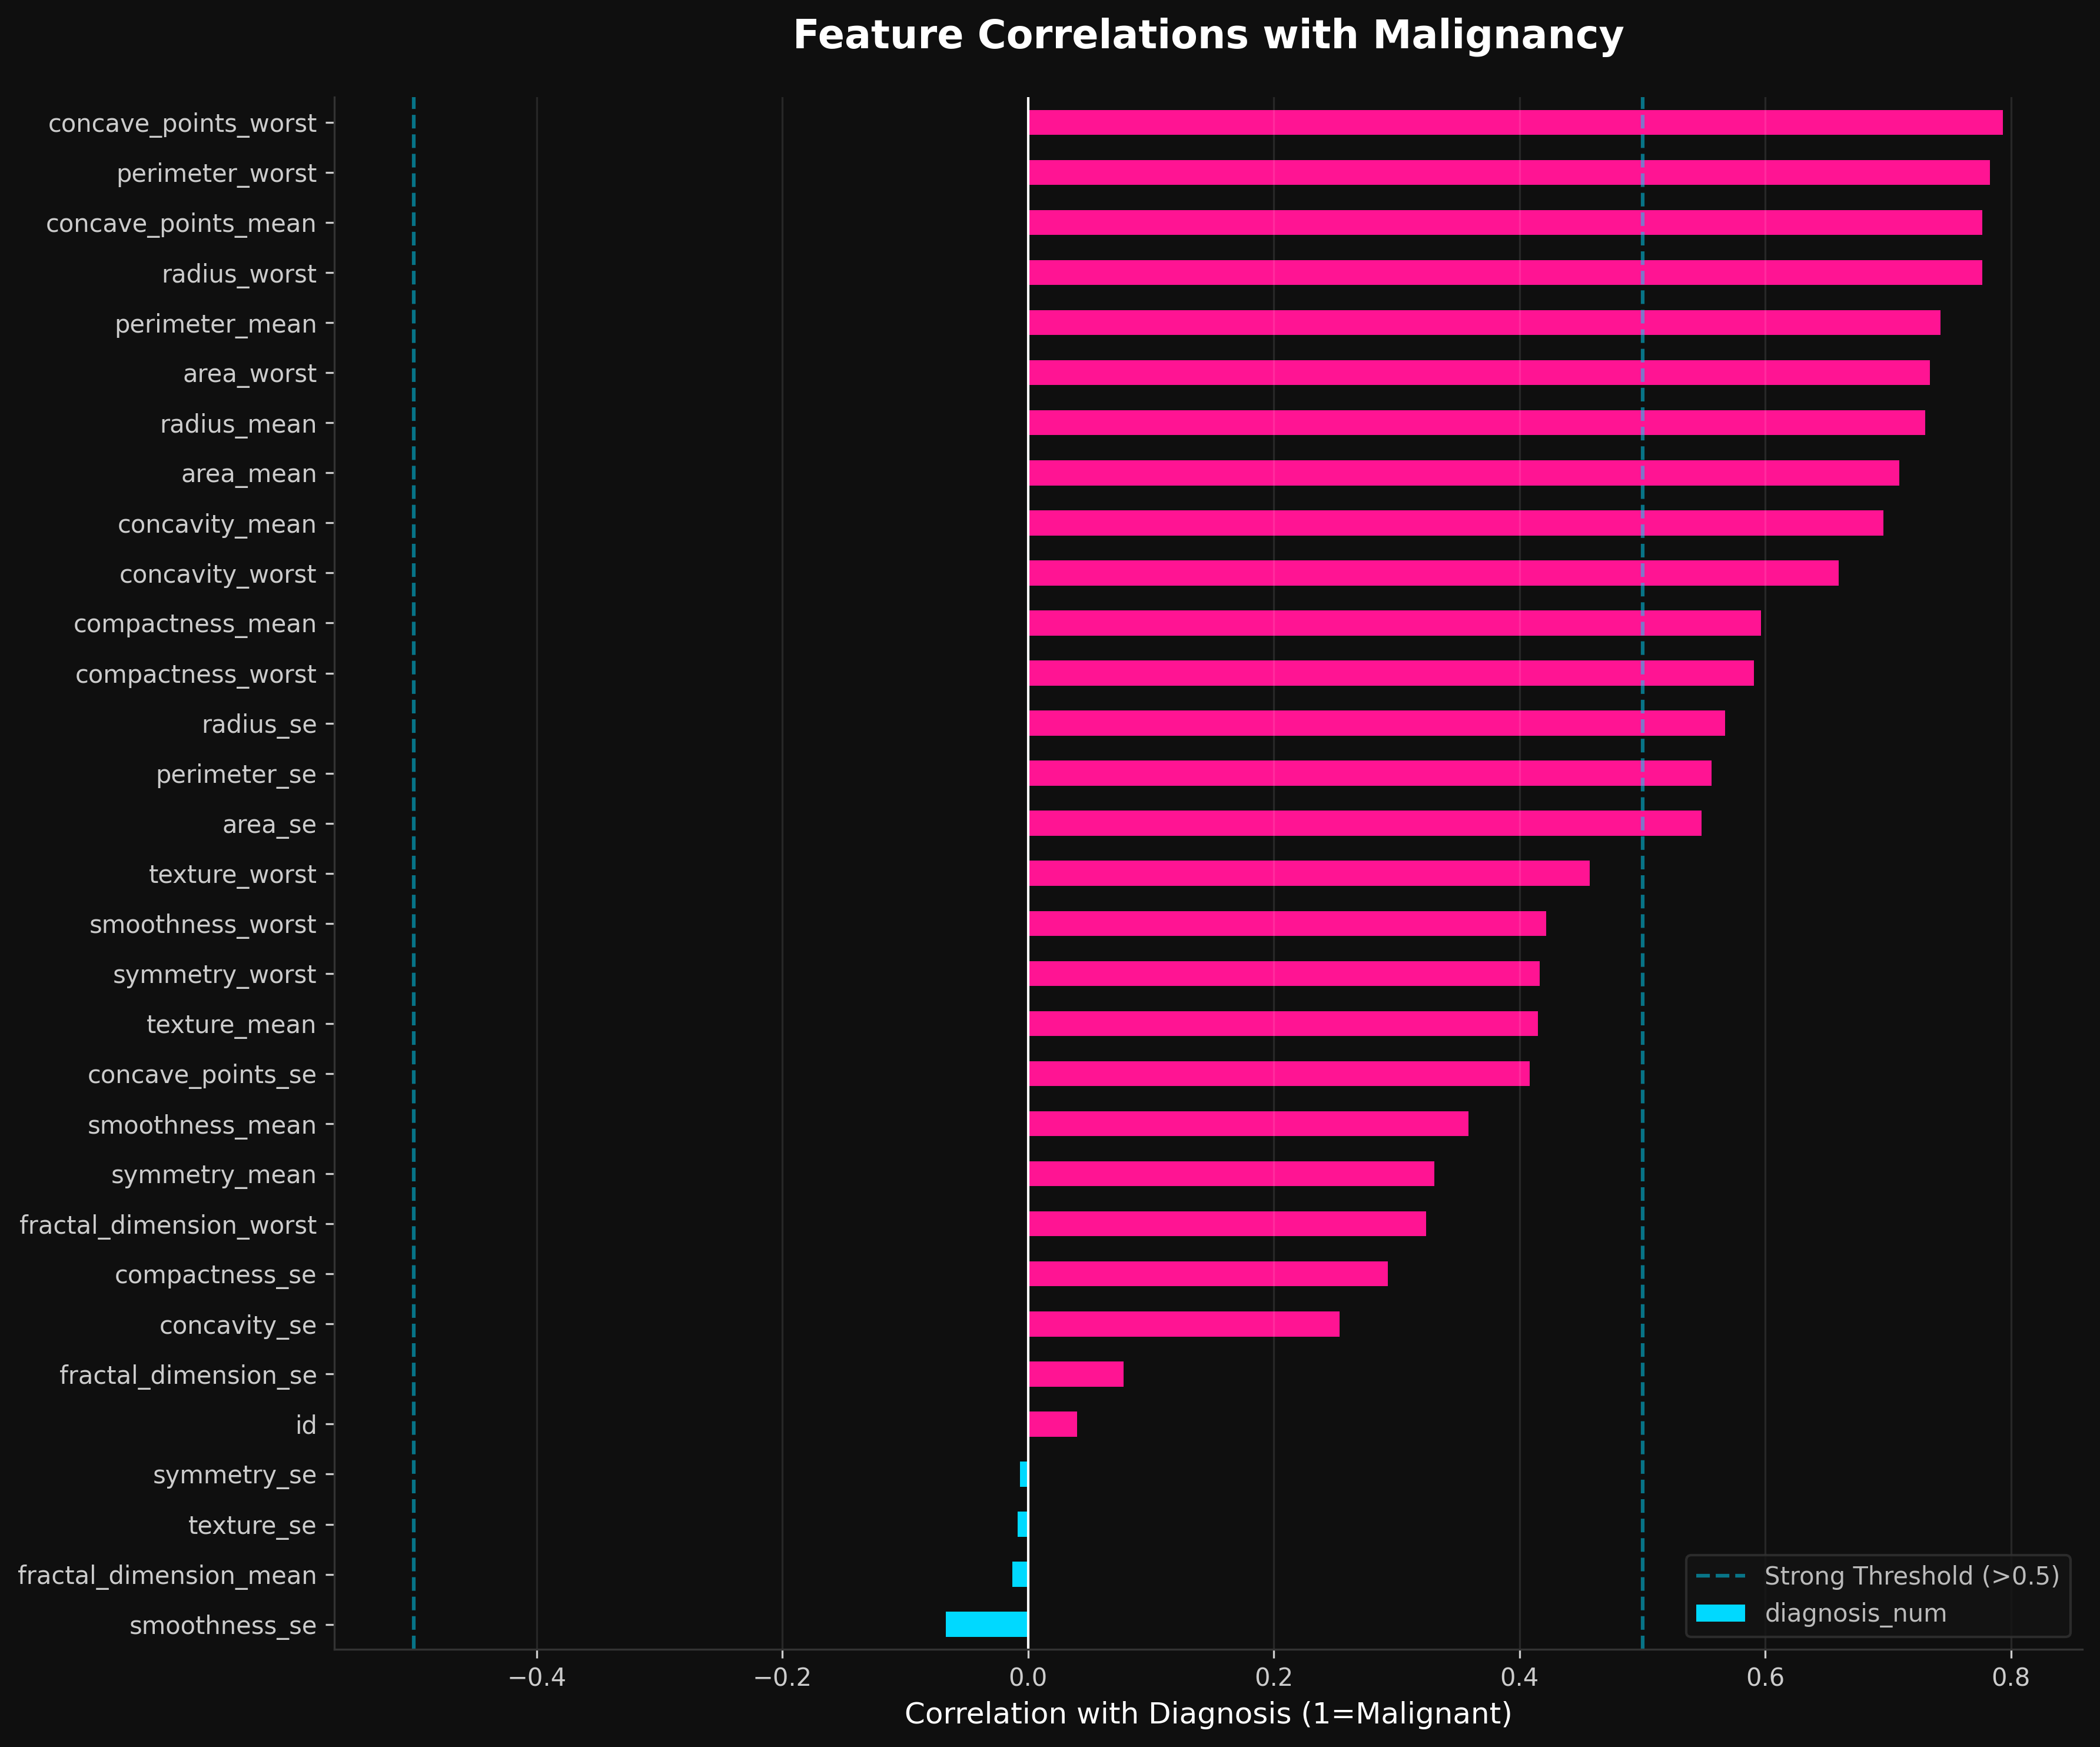
\includegraphics[width=0.6\textwidth]{images/wbcd_correlation_barh.png}
    \caption{Feature Correlations with Malignancy}
    \label{fig:wbcd_corr_barh}
\end{figure}

The horizontal bar chart highlights features with the strongest influence:
\begin{itemize}
    \item \textbf{Positive Correlation (Pink):} Features like \texttt{concave points\_worst}, \texttt{perimeter\_worst}, and \texttt{radius\_worst} show very strong positive correlation ($> 0.7$) with malignancy. Larger, more irregular nuclei are strong indicators of cancer.
    \item \textbf{Negative Correlation (Cyan):} Some texture and fractal dimension features show weaker or negative correlations.
\end{itemize}
High multicollinearity is also observed among geometric features (e.g., Radius, Perimeter, Area), suggesting that dimensionality reduction or regularization (e.g., L2 penalty) could be beneficial.

\subsection{METABRIC Exploratory Data Analysis}
The \textbf{Molecular Taxonomy of Breast Cancer International Consortium (METABRIC)} dataset was analyzed following a structured approach to understand the underlying distributions and relationships before modeling.

\subsubsection{Dataset Overview}
The METABRIC dataset serves as the foundation for the prognosis prediction tasks. It combines clinical attributes with detailed genomic profiles to enable multi-faceted patient evaluation.
\begin{itemize}
    \item \textbf{Instances:} 1,904 patients.
    \item \textbf{Features:} Clinical variables (e.g., Age, Tumor Size, Lymph Nodes) and genomic markers.
    \item \textbf{Objective:} To predict tumor aggressiveness, growth rate, and 6-month evolution status.
\end{itemize}

\subsubsection{Missing Value Analysis}
Data quality is critical for reliable regression modeling. The missing value analysis reveals a generally high-quality dataset, though some imputation is required.

\begin{figure}[H]
    \centering
    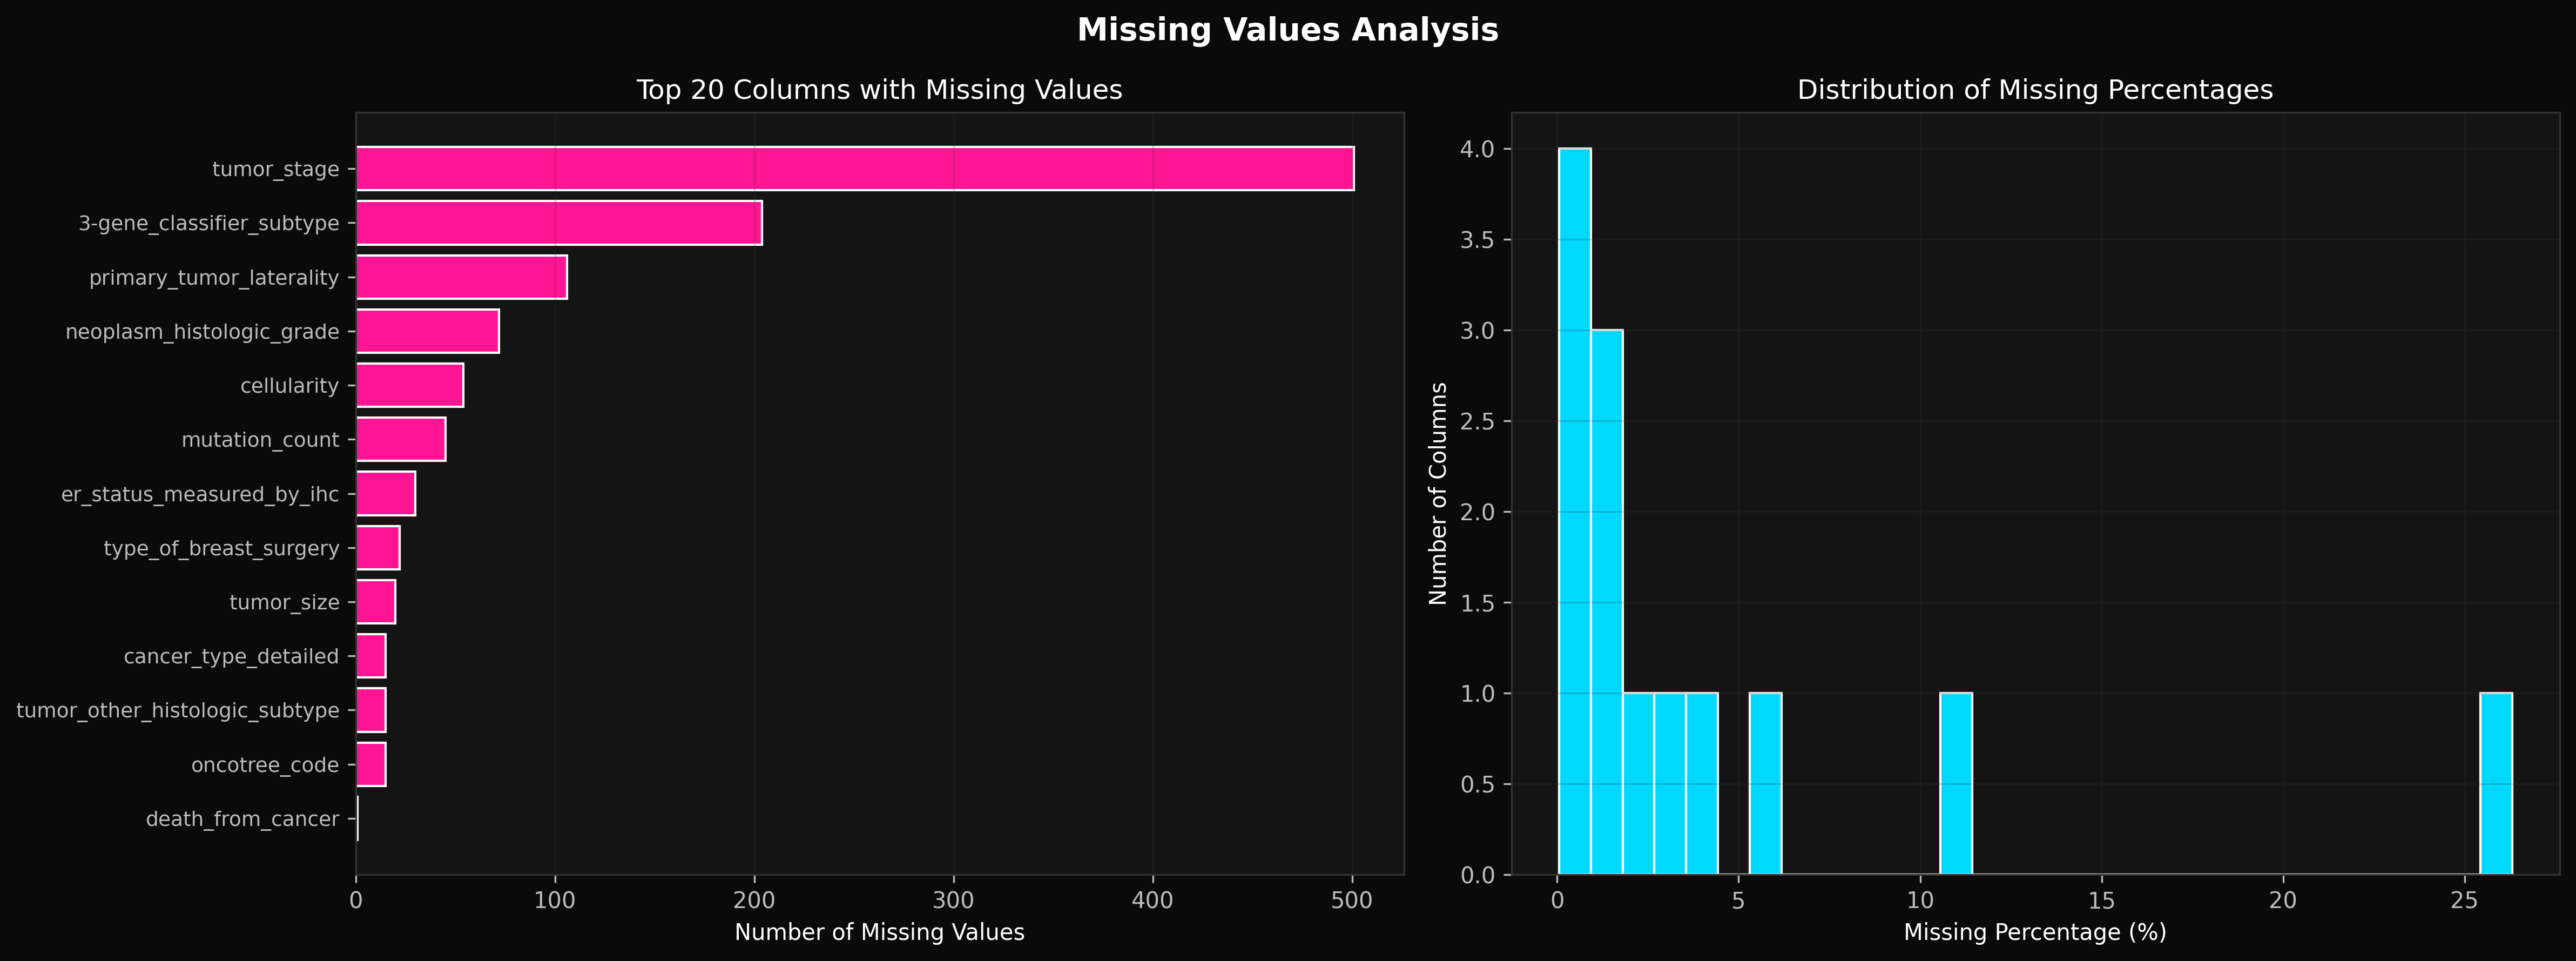
\includegraphics[width=\textwidth]{images/metabric_missing_values.png}
    \caption{Missing Value Analysis: Top Columns and Distribution}
    \label{fig:metabric_missing}
\end{figure}

The visualization highlights that while most columns are complete, specific clinical features (e.g., \texttt{tumor\_stage}, \texttt{tumor\_size}) contain missing entries that must be addressed during preprocessing.

\subsubsection{Clinical Variable Statistics}
Key statistical measures for the primary clinical features are summarized below.

\begin{table}[H]
\centering
\renewcommand{\arraystretch}{0.9}
\scalebox{0.92}{
\begin{tabular}{|l|c|c|c|c|}
\hline
\textbf{Feature} & \textbf{Mean} & \textbf{Std Dev} & \textbf{Min} & \textbf{Max} \\ \hline
age\_at\_diagnosis & 61.087 & 12.979 & 21.930 & 96.290 \\ \hline
tumor\_size & 25.075 & 10.780 & 1.000 & 49.500 \\ \hline
nottingham\_prognostic\_index & 4.033 & 1.144 & 1.000 & 6.360 \\ \hline
lymph\_nodes\_examined\_positive & 1.295 & 1.770 & 0.000 & 5.000 \\ \hline
mutation\_count & 5.681 & 4.012 & 1.000 & 80.000 \\ \hline
overall\_survival\_months & 125.121 & 76.334 & 0.000 & 355.200 \\ \hline
\end{tabular}
}
\caption{Descriptive Statistics for METABRIC Clinical Features}
\label{tab:metabric_stats}
\end{table}

\subsubsection{Numerical Variable Distribution}
The distributions of continuous variables provide insights into the patient population demographics and tumor characteristics.

\begin{figure}[H]
    \centering
    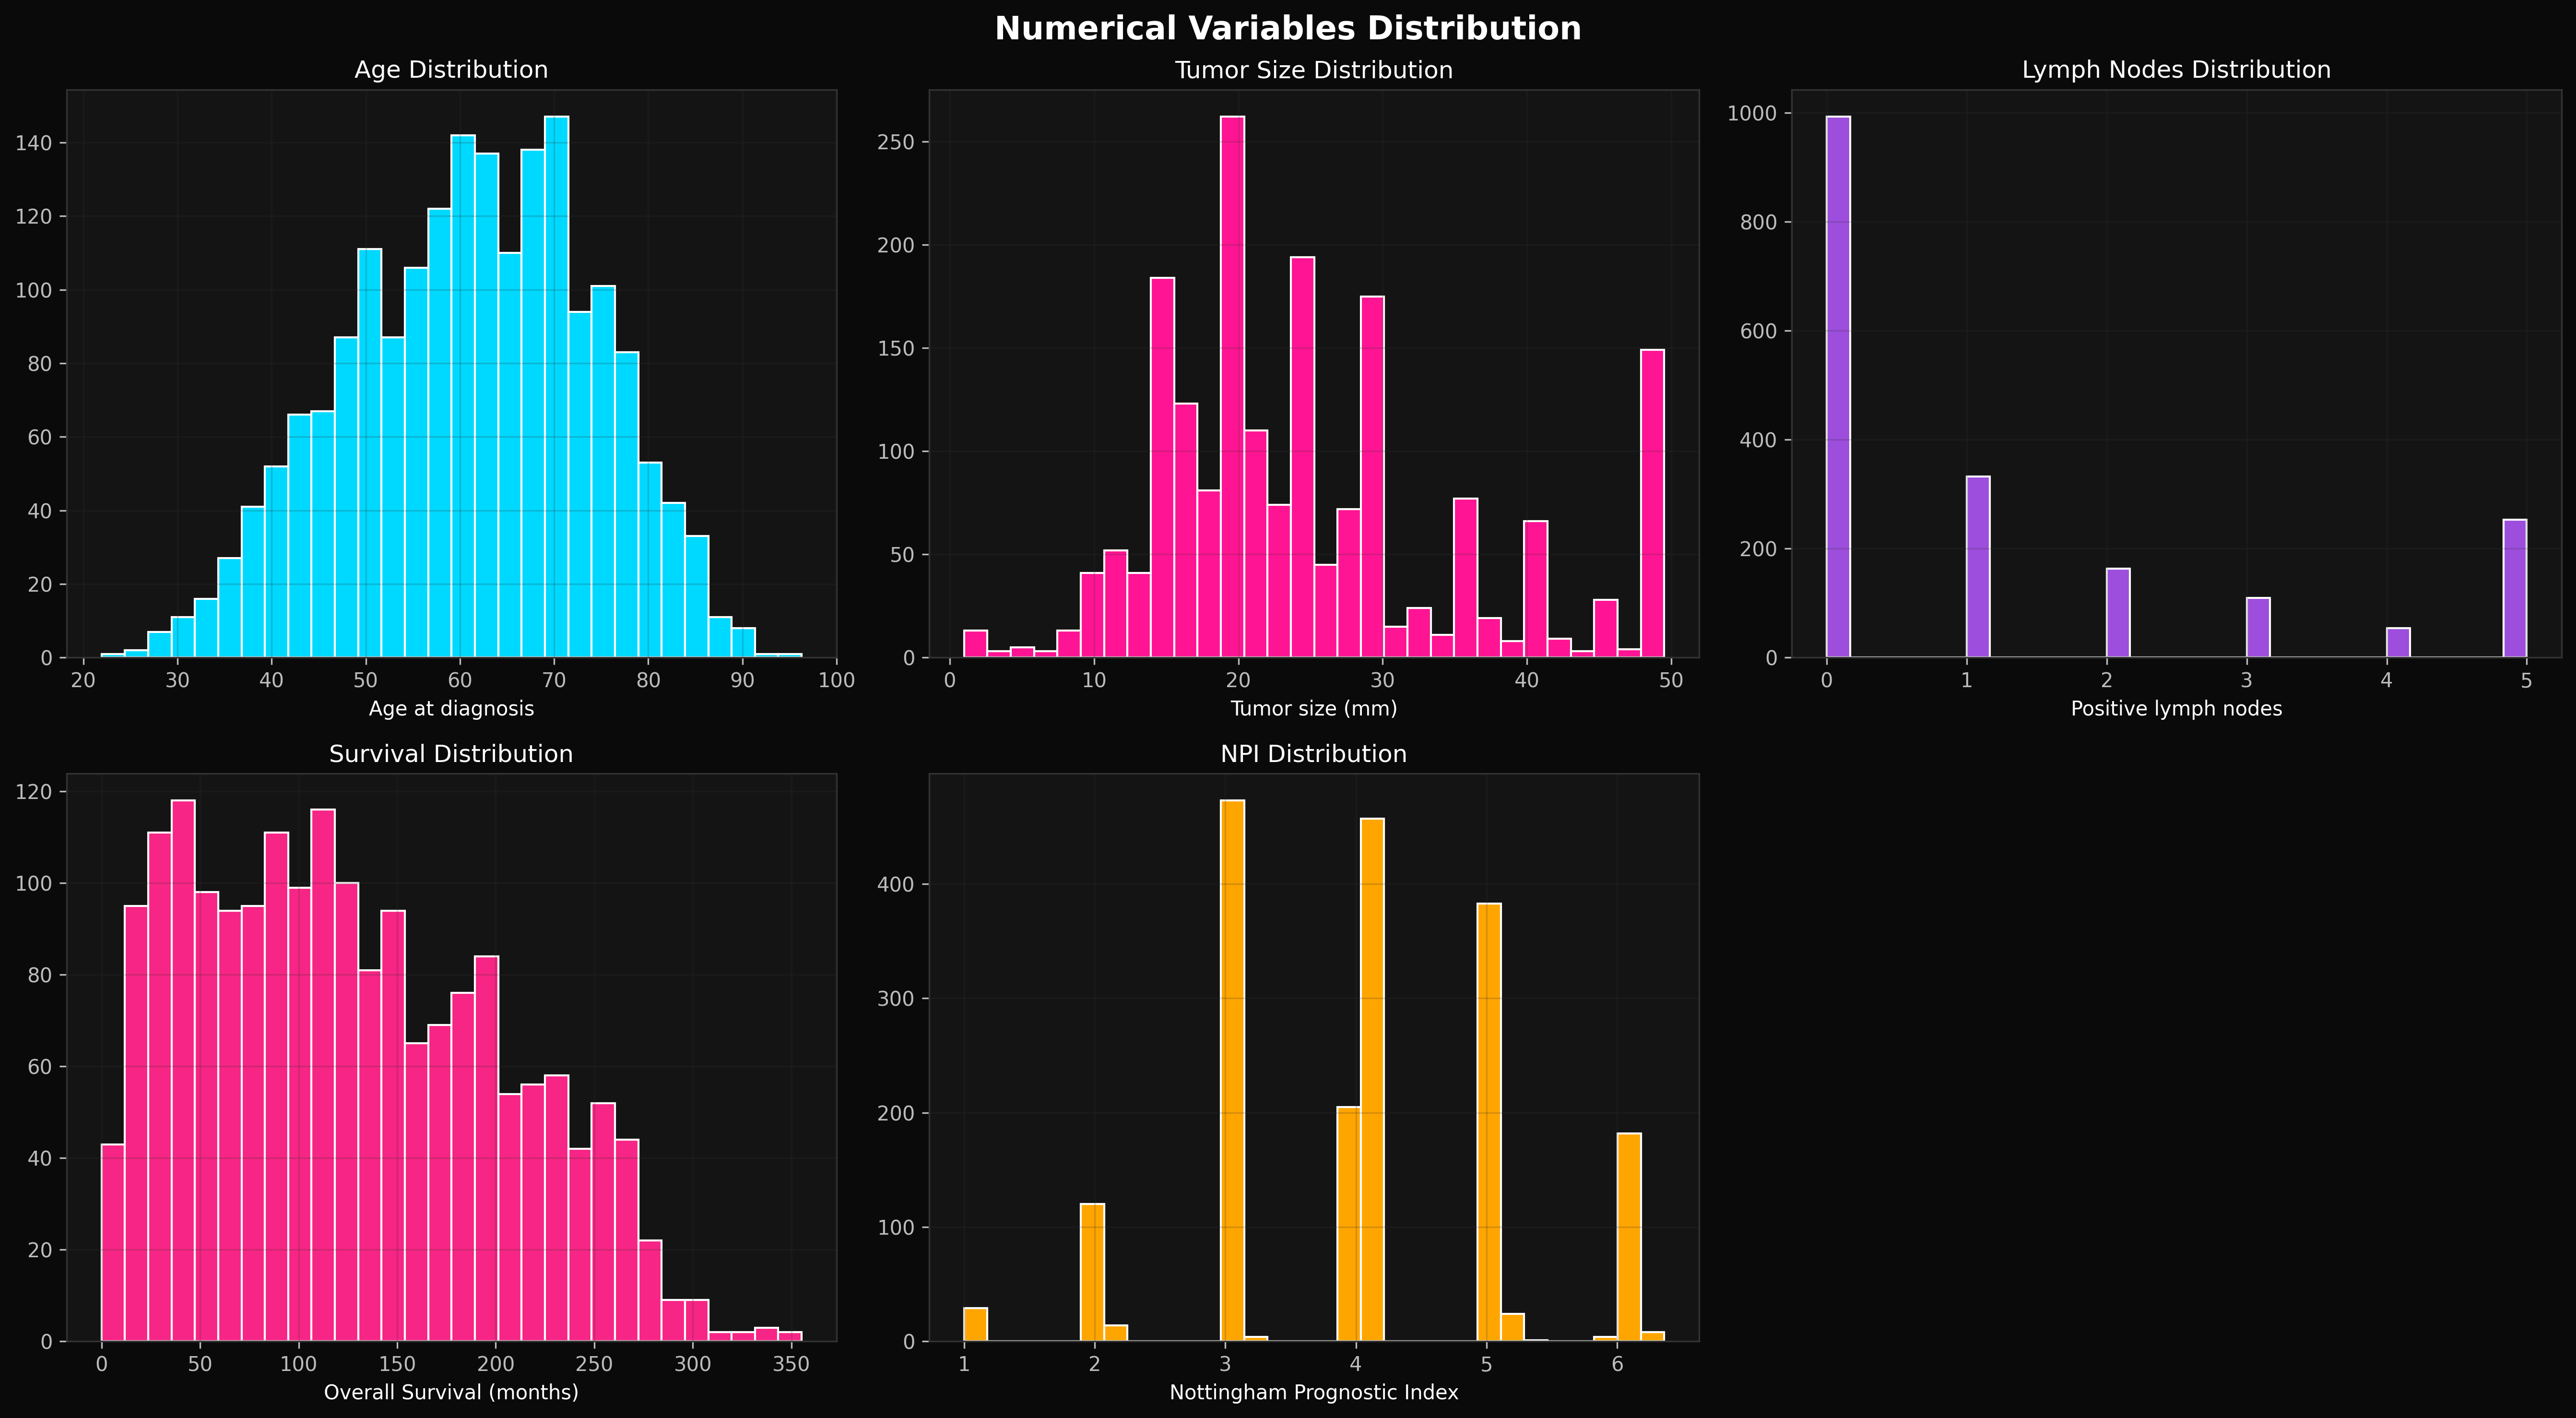
\includegraphics[width=\textwidth]{images/metabric_numerical_dist.png}
    \caption{Distribution of Numerical Clinical Variables}
    \label{fig:metabric_numerical}
\end{figure}

\begin{itemize}
    \item \textbf{Age:} The age distribution is roughly normal, centered around 60 years.
    \item \textbf{Tumor Size:} Shows a right-skewed distribution, indicating most tumors are detected at a smaller size.
    \item \textbf{Lymph Nodes:} Highly right-skewed, with most patients having few positive nodes.
    \item \textbf{Survival Months:} A wide distribution reflecting the variable nature of breast cancer prognosis.
\end{itemize}

\subsubsection{Categorical Variables Distribution}
Categorical features such as histologic grade and tumor stage are essential for risk stratification.

\begin{figure}[H]
    \centering
    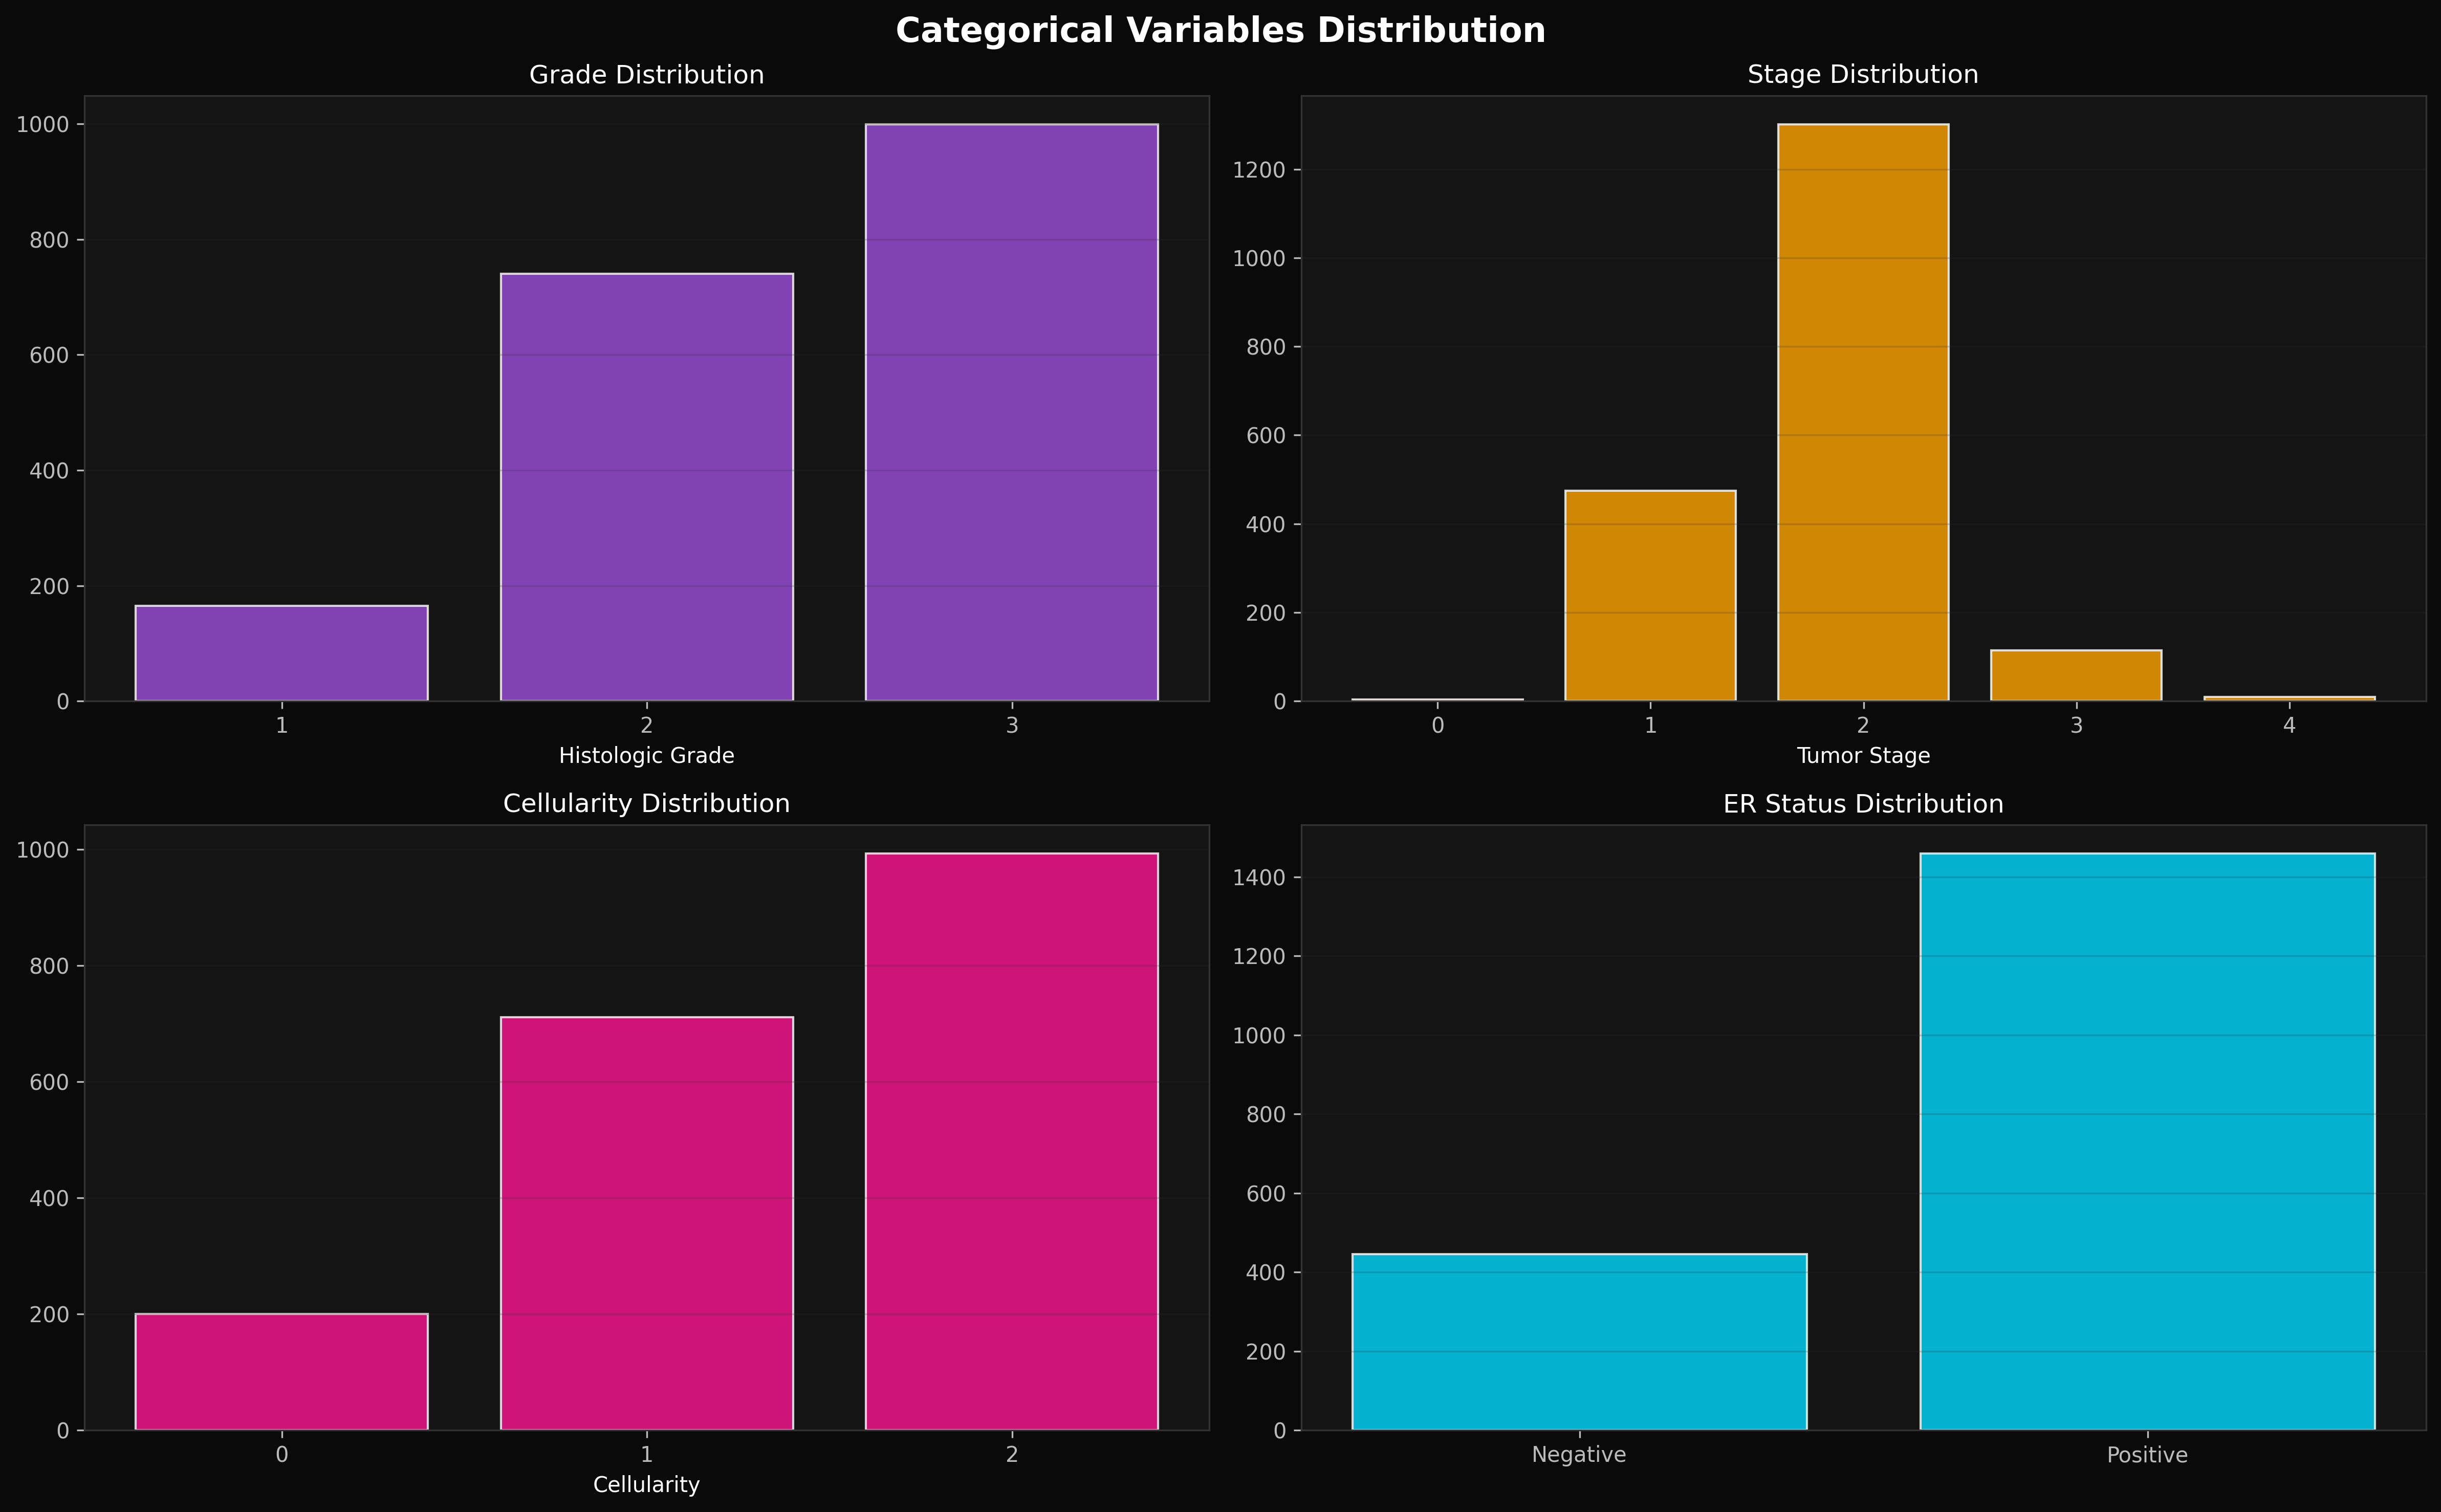
\includegraphics[width=0.7\textwidth]{images/metabric_categorical_dist.png}
    \caption{Distribution of Categorical Clinical Variables}
    \label{fig:metabric_categorical}
\end{figure}

The plots reveal the prevalence of different cancer grades and stages, which are direct inputs into the Aggressiveness Score calculation.

\subsubsection{Correlation Analysis}
To understand the interdependencies between clinical variables, a correlation matrix was generated.

\begin{figure}[H]
    \centering
    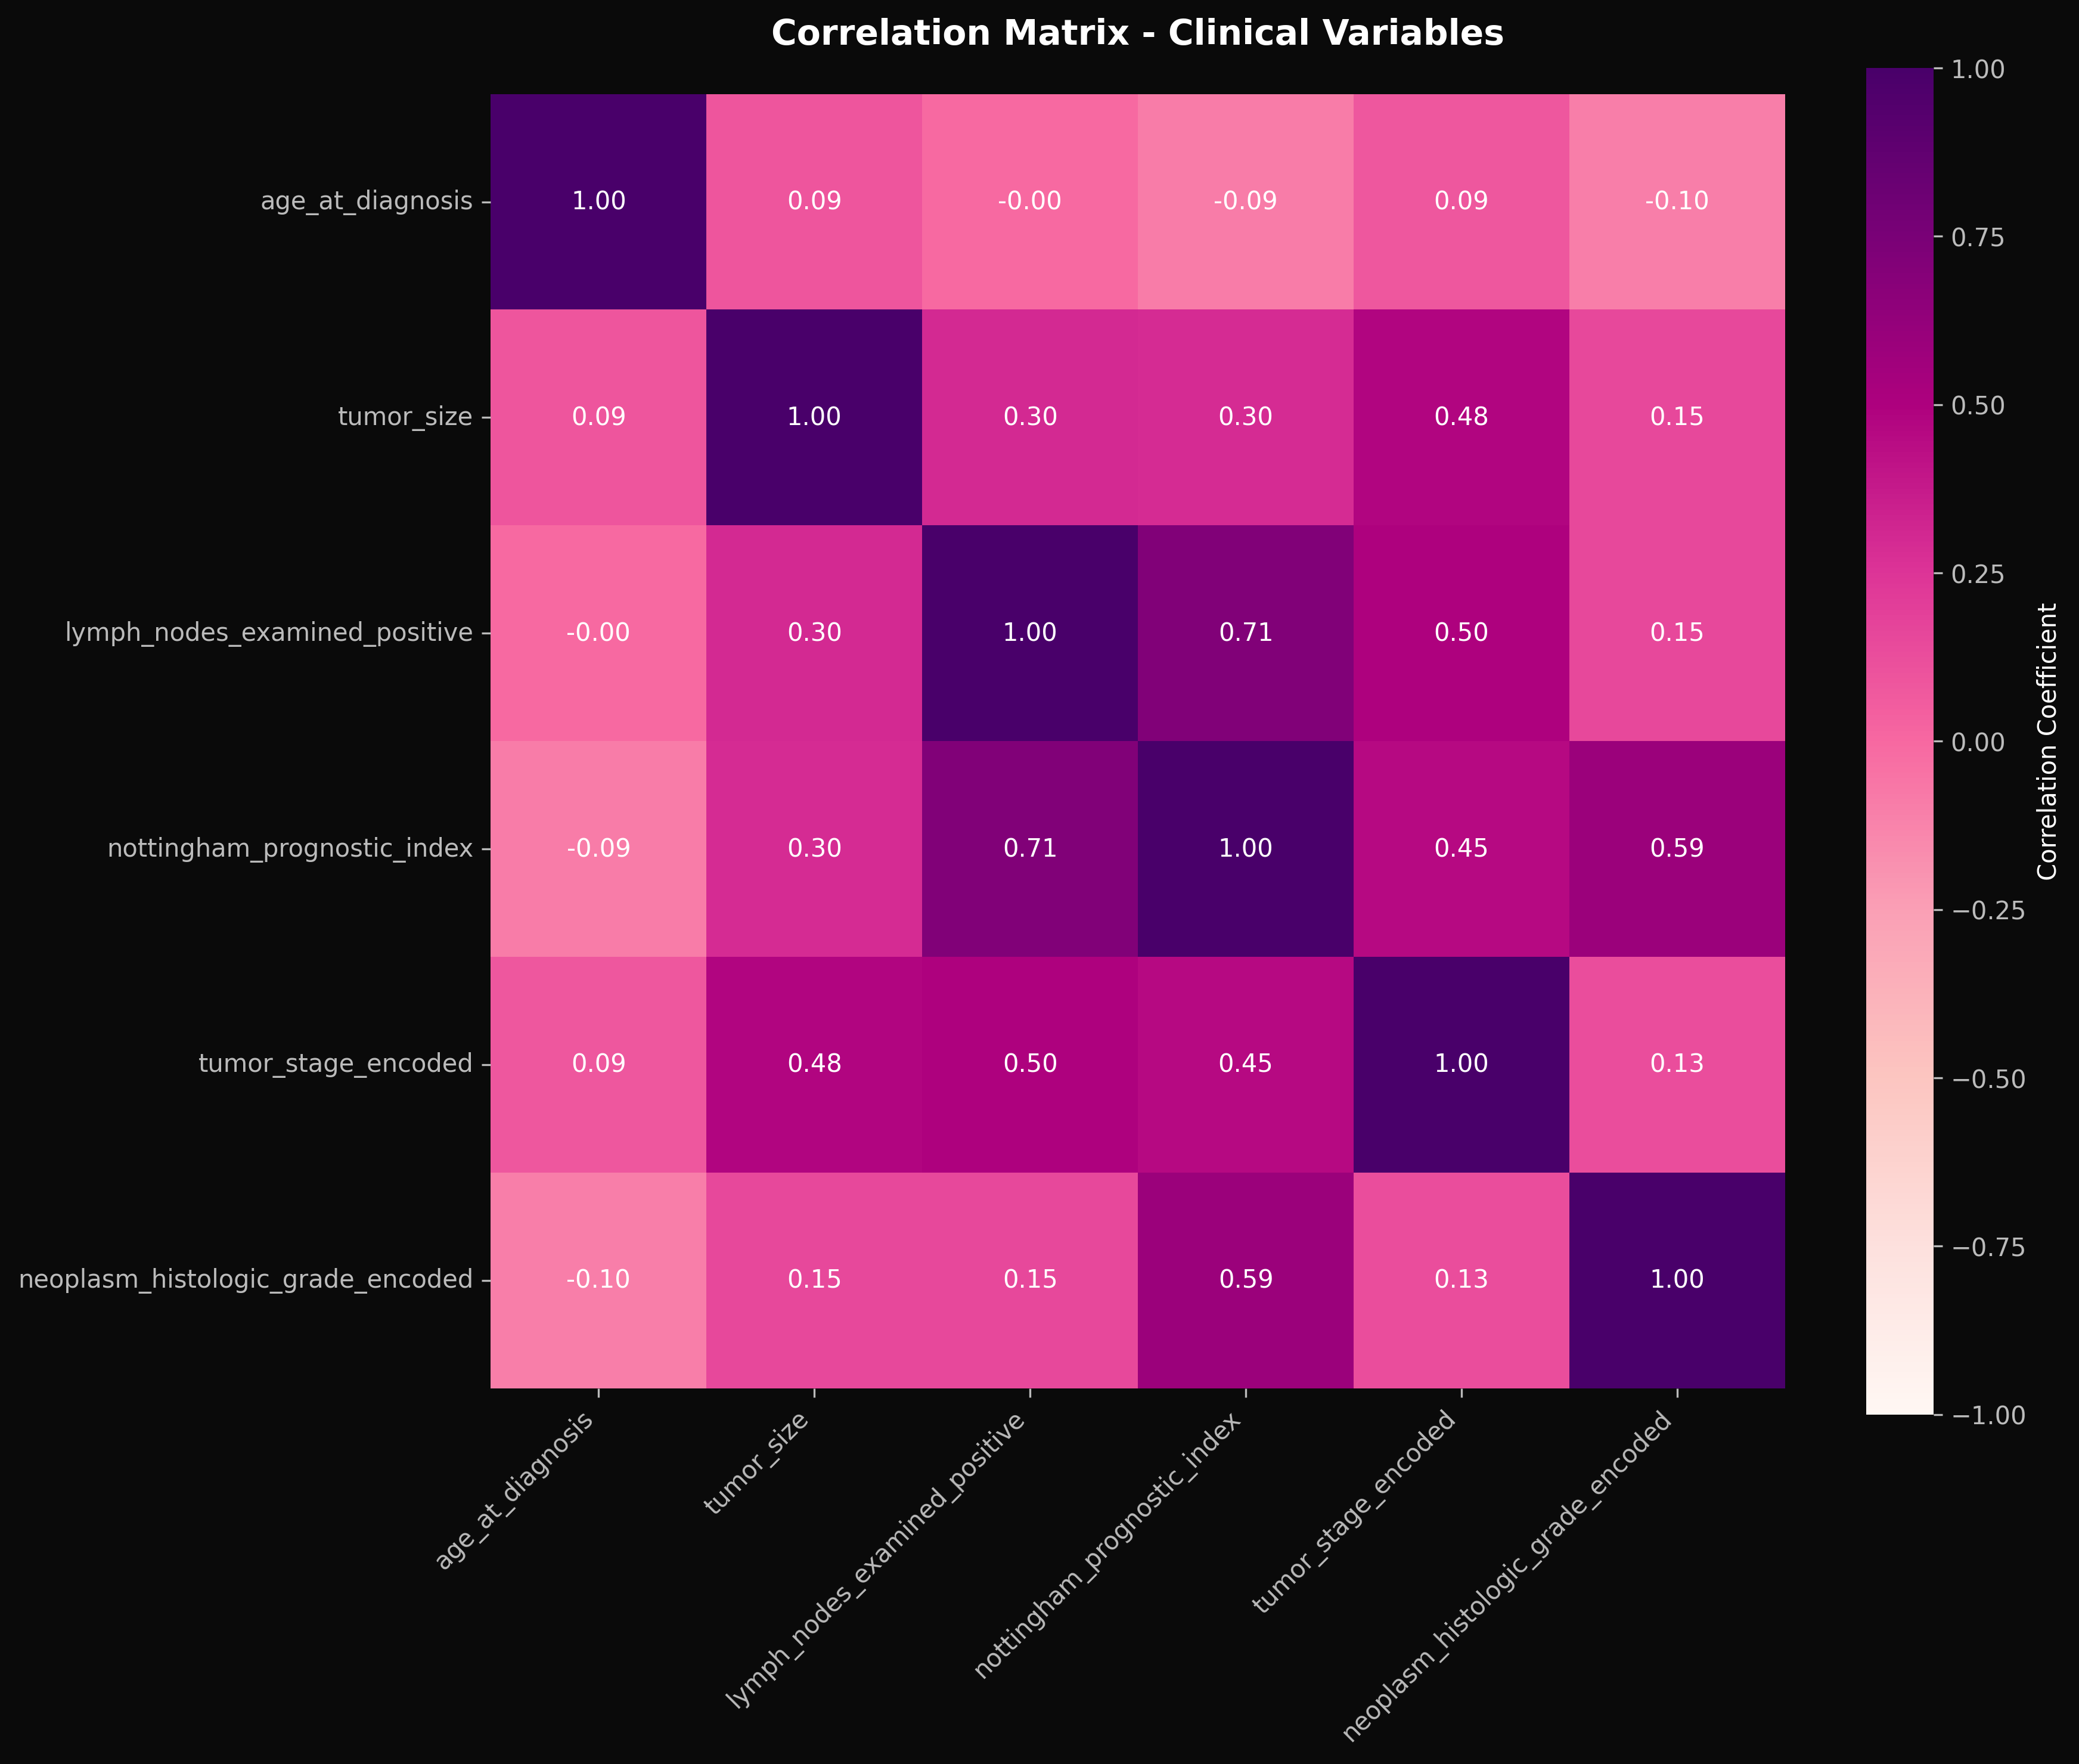
\includegraphics[width=0.5\textwidth]{images/metabric_correlation.png}
    \caption{Correlation Matrix of Clinical Variables}
    \label{fig:metabric_corr}
\end{figure}

\begin{itemize}
    \item \textbf{NPI \& Grade:} Strong positive correlation, as NPI is mathematically derived from grade.
    \item \textbf{Tumor Size \& Stage:} Positive correlation, as larger tumors typically correspond to advanced stages.
    \item \textbf{Nodes \& NPI:} Significant correlation, reinforcing the NPI as a composite measure of severity.
\end{itemize}
